\documentclass{appolb}
\usepackage{bigints}
\usepackage{tikz}

\usepackage{graphicx}
\usepackage{bigints}

\usepackage{tabularx}
\usepackage{graphics}
\usepackage{subfig}
\usepackage{xcolor}
\usepackage{array}

\usepackage{cite}
\usepackage{placeins}


% graphicx package included for placing figures in the text
%------------------------------------------------------

%%Additional libraries added by authors==========================
\usepackage{amsmath}
%%

%%Author Short hands==========================
\newcommand{\dd}{\text{d}}
\newcommand{\ttb}{\text{t} \bar{\text{t}} }
\newcommand{\txt}{\text{t} }
\newcommand{\dis}{\displaystyle}
\newcommand{\txtb}{\bar{\text{t}} }
\newcommand{\Bf}[1]{\mathbf{#1}}
\newcommand{\pvec}[1]{\vec{#1}\mkern2mu\vphantom{#1}}


%==========================================
%Definitions for the use of tikz
\usepackage{tikz}
\usetikzlibrary{arrows}
\usetikzlibrary{shapes,matrix}
\usetikzlibrary{patterns}
\usetikzlibrary{shapes.misc}
\usetikzlibrary{trees}
\usetikzlibrary{decorations.pathreplacing}
\usetikzlibrary{decorations.pathmorphing}
\usetikzlibrary{decorations.markings}
\usepackage{tikz,ifthen}% TikZ!
\tikzset{beamerprimary/.style={structure.fg, thick}}
\tikzset{beamersecondary/.style={structure.bg, thick}}
%For Feynman diagrams
\tikzset{
boson/.style={decorate, decoration={snake,amplitude=1.2pt, segment length=2.5pt}},
    gluon/.style={decorate, 
        decoration={coil,amplitude=2pt, segment length=2.5pt}},
gluonb/.style={color=black,decorate, 
        decoration={coil,amplitude=1.2pt, segment length=2.5pt}},  
gluonr/.style={color=red,decorate, 
        decoration={coil,amplitude=1.2pt, segment length=2.5pt}},
    scalar/.style={densely dashed},
gluono/.style={decorate, 
        decoration={coil,amplitude=1.3pt, segment length=2pt}},
gluonbl/.style={color=blue,decorate, 
        decoration={coil,amplitude=1.2pt, segment length=2.5pt}},  
    plain/.style={double},	
cross/.style={cross out,draw,minimum size=2*(#1-\pgflinewidth), 
         inner sep=0pt,outer sep=0pt},
         %default radius will be 1pt. 
        cross/.default={1pt},
           zz/.style={decorate, 
        decoration={zigzag,amplitude=2pt, segment length=4pt}},
         fermion/.style={postaction={decorate},
        decoration={markings,mark=at position .55 with {\arrow{>}}}},
         parton/.style={postaction={decorate},
        decoration={markings}}, 
    gluon/.style={decorate, 
        decoration={coil,amplitude=2pt, segment length=4pt}},
     ghost/.style={draw=black,dashed,postaction={decorate},
        decoration={markings,mark=at position .55 with {\arrow{>}}}},
        higgs/.style={draw=black,dashed},
}


\tikzstyle{every node}=[font=\footnotesize]
\tikzstyle{lwg} = [line width=1.2pt]
\tikzstyle{lwd} = [line width=0.8pt]
\tikzstyle{twide} = [line width=0.4pt]
%%%%%%%==========================


%%
%%%%%%%%%%%%%%%%%%%%%%%%%%%%%%%%%%%%%%%%%%%%%%%%%%
%                                                %
%    BEGINNING OF TEXT                           %
%                                                %
%%%%%%%%%%%%%%%%%%%%%%%%%%%%%%%%%%%%%%%%%%%%%%%%%%
\begin{document}
% \eqsec  % uncomment this line to get equations numbered by (sec.num)
\title{A new approach to top pair production at NNLO%
\thanks{
Work in collaboration with Micha\l{} Czakon and Sebastian Sapeta.
Presented at the XXXIX International Conference of Theoretical Physics ``Matter to the
Deepest'' 2017, Podlesice, Poland, September 2017.}%
% you can use '\\' to break lines
}
\author{Ren\'e \'Angeles-Mart\'inez
\address{H. Niewodnicza\'{n}ski Institute of Nuclear Physics, Radzikowskiego 152, Krak\'ow, Poland}
\\[1.5ex]
{
}
%Micha\l{} Czakon
%\address{Institut f\"{u}r Theoretische Teilchenphysik und Kosmologie, RWTH Aachen University, D-52056 Aachen, Germany}
}
\maketitle%
\begin{abstract}
We report progress on a new approach to calculate  top pair production cross-sections at NNLO. This consists in combining the slicing method with the soft collinear effective theory. The necessary matrix elements already exist in the literature except for soft function at NNLO. We describe a strategy to evaluate this function numerically, and make a robust validation against the renormalisation group and our analytic results.   

 \end{abstract}
\PACS{12.38.Bx}
  
\section{Introduction}
Top pair ($\ttb$) production is relevant for searches of new physics at the LHC \cite{Czakon:2015xqa}. With the experiment providing highly precise data, the community is motivated to strengthen the current theoretical understanding of this process.  Some important aspects that are currently being studied are the top mass definition, its decay modelling and the  perturbative QCD corrections. Here we focus on the latter. 
At the moment, only one group has calculated the full total and differential QCD corrections at NNLO
 \cite{Czakon:2013goa,Czakon:2015owf,Czakon:2017wor} and other groups have reported partial results 
\cite{Abelof:2015lna,Abelof:2014jna,Bonciani:2015sha} that agree at the level of the total cross-section. In addition, there are various approximate results at this order, see Refs. \cite{Ahrens:2010zv,Ahrens:2011mw,Kidonakis:2012rm,Kidonakis:2014pja,Gao:2012ja,Brucherseifer:2013iv}. 
%Detailed comparisons are not yet available; these require dedicated work to single out or approximate accordingly.

In this proceedings, we report progress on a new approach to evaluate a wide-range of differential cross-sections at NNLO. 
We have the two-fold motivation of  providing a full independent test of such cross-sections and of developing an approach that 
can be applied to other processes at high orders, \emph{e.g.} $gg\to H$ at N$^3$LO. The approach brings together various tested 
strategies in the literature:
\begin{enumerate}
\item Firstly, we use the key observation of the slicing method \cite{Bonciani:2015sha,Catani:2007vq} that a cross-section $\sigma^{\text{NNLO}}_{\ttb}$ integrated over the transverse momentum of the  $\ttb$ pair, $q_T$, can be written as
\begin{align}
\sigma^{\text{NNLO}}_{\ttb}=
\int\displaylimits_{q_T < q_{T\text{cut}}} \!\!\!\! \dd q_T  
\frac{\dd \sigma^{\text{NNLO}}_{\ttb} }{\dd q_T}+
\int\displaylimits_{q_T > q_{T\text{cut}}}\!\!\!\! \dd q_T  
\frac{\dd \sigma_{\ttb}^{\text{NLO+jet}}}{\dd q_T}~.
 \label{eq:master}
\end{align} 
The second term on the right-hand-side is well known, see for example \cite{Dittmaier:2007wz,Dittmaier:2008uj}. 
\item Secondly, to calculate the small-$q_T$ region ($q_T<q_{T\text{cut}}$),  we adopt Soft Collinear Effective Theory (SCET), which has been applied to same process at NLO \cite{Li:2013mia}. All the relevant SCET operators except the soft function are  know up at NNLO. 
\item Finally, the graphs contributing to the soft function at NNLO have a common structure that can be algorithmically evaluated using a numerical approach. 
\end{enumerate}
In the following sections, we discuss points 2 and 3 from this list and in Sec.~\ref{sec:validation} we validate our algorithm by cross-checking against the contributions involving fermions: a part of the NNLO soft function that, by itself, can be compared against the SCET renormalisation group  and that we have been able to evaluate analytically. 



\section{SCET for the small-$q_T$ region}
Let us denote by $p_1$ and $p_2$ the momenta of the incoming partons that interact to produce a pair of top quarks with momenta $p_\txt$ and $p_{\txtb}$, plus additional partonic radiation $X$, \emph{i.e.} we are interested in the process
\begin{align}
\text{q}(p_1)+\bar{\text{q}}(q_2)\to \txt(p_{\txt})+ \bar{\txt} (p_{\txtb})+X~.
\end{align}
The SCET framework  ascertains \cite{Li:2013mia}, first, that when the  momentum of the top pair $q= p_\txt+p_{\txtb}$ satisfies
\begin{align}
\Lambda_{QCD}\ll q_T^2\ll q^2, m_\txt^2 ,(p_1+p_2)^2, (p_1-p_{\txt})^2-m_\txt^2, (p_1-p_{\txtb})^2-m_\txt^2, 
\end{align}
the states, $X$, which are not power suppressed\footnote{$\Lambda^2/q_T^2$ or $\Lambda^2/q^2$.} have momentum $(k^{\pm},k^{\mp},k_T^\mu)$ that is either hard $k\sim(1,1,1)$, soft $k\sim(\lambda,\lambda,\lambda)$ or collinear $k\sim(\lambda^2,1,\lambda)$, where $\lambda=\Lambda/q_T$ and,  second, that the cross-section can be written as the convolution of the hard ($\mathbf {H}_{i\bar{i}}$),  soft ($\mathbf {S}_{i\bar{i}}$) and beam ($B_i$)  functions  that respectively describe the physics of these regions. Schematically, this can be written as
\begin{align}
  &\frac{d\sigma_{\ttb}}{\dd q_T^2 \, \dd y \, \dd q^2 \, \dd \! \cos\theta} = 
 \sum_X 
%  \\& 
  \sum_{i = \text{q},\bar{\text{q}},\text{g} }   
%  \left( \frac{x_\perp^2q^2}{4e^{-2\gamma_E}} \right)^{-F_{i \bar{i}}( x_\perp^2\mu^2)} 
B_{i} (\xi_1, x_T,\mu) \,  \otimes\, 
B_{\bar{i}}(\xi_2, x_T,\mu)\, \otimes\nonumber  \\
&   \text{Tr} 
  \big[\,  \mathbf {H}_{i\bar{i}}(q^2,m, v_\txt ,\mu)  
  \otimes  \mathbf {S}_{i\bar{i}}(x_T, v_t ,\mu)  \big]. \label{eq:Factorisation}
\end{align}
Here  $\mu$ is the factorisation scale, the sum over $i$ runs over the possible production channels and the convolution should be understood over the longitudinal factions $\xi_i$ and the transverse coordinates $x_\perp$. The kinematical variables $y$ and $v_{\txt}$ are defined in the the $\ttb$ rest frame, $y$ is the rapidity of $\ttb$ pair and 
\begin{align}
p_\txt=m_{\txt}(1-\beta^2)^{-1} (1,\beta v_\txt),\qquad  v_\txt= \beta(\cos\theta  ,\sin\theta\, \hat{n}_T), 
\end{align}
where $\beta= \sqrt{1-4 m^2_\txt/q^2}$ is the velocity of $p_\txt$. We refer the reader to Refs.~\cite{Li:2013mia,Gehrmann:2014yya} for a detailed presentation of this expression. 

In SCET, the  soft, hard and beam functions have perturbative expansions, each of which  is potentially simpler than the expression for the 
complete cross-section. In the case of Eq.~\eqref{eq:Factorisation}, the hard function and the process-independent beam functions \cite{Gehrmann:2012ze,Gehrmann:2014yya} are known up to NNLO but the soft function is only known up to NLO\cite{Li:2013mia}.

\section{Integration strategy of the soft function at NNLO}


We work in momentum space,  $ \Bf{S}_{i\bar{i}}(q'_T, v_t ,\mu)$, where the soft function amounts to a product of Wilson lines with soft emissions having a fixed total transver momenta, $q'_T$. Up to NNLO, the integration of the azimuthal angle of  $x_T$ commutes to the right of  the beam and hard functions,  and acts only on the soft function \cite{Li:2013mia}. Remarkably, at each order in $\alpha_s$, such azimuthal integration can be used to factor away the $q'_T$ dependence\footnote{Hence, the integration in momentum and coordinates space can be easily related to each other.}.  We illustrate all this in  Fig.~\ref{fig:soft_function}.
\begin{figure}[htb]
\centering{
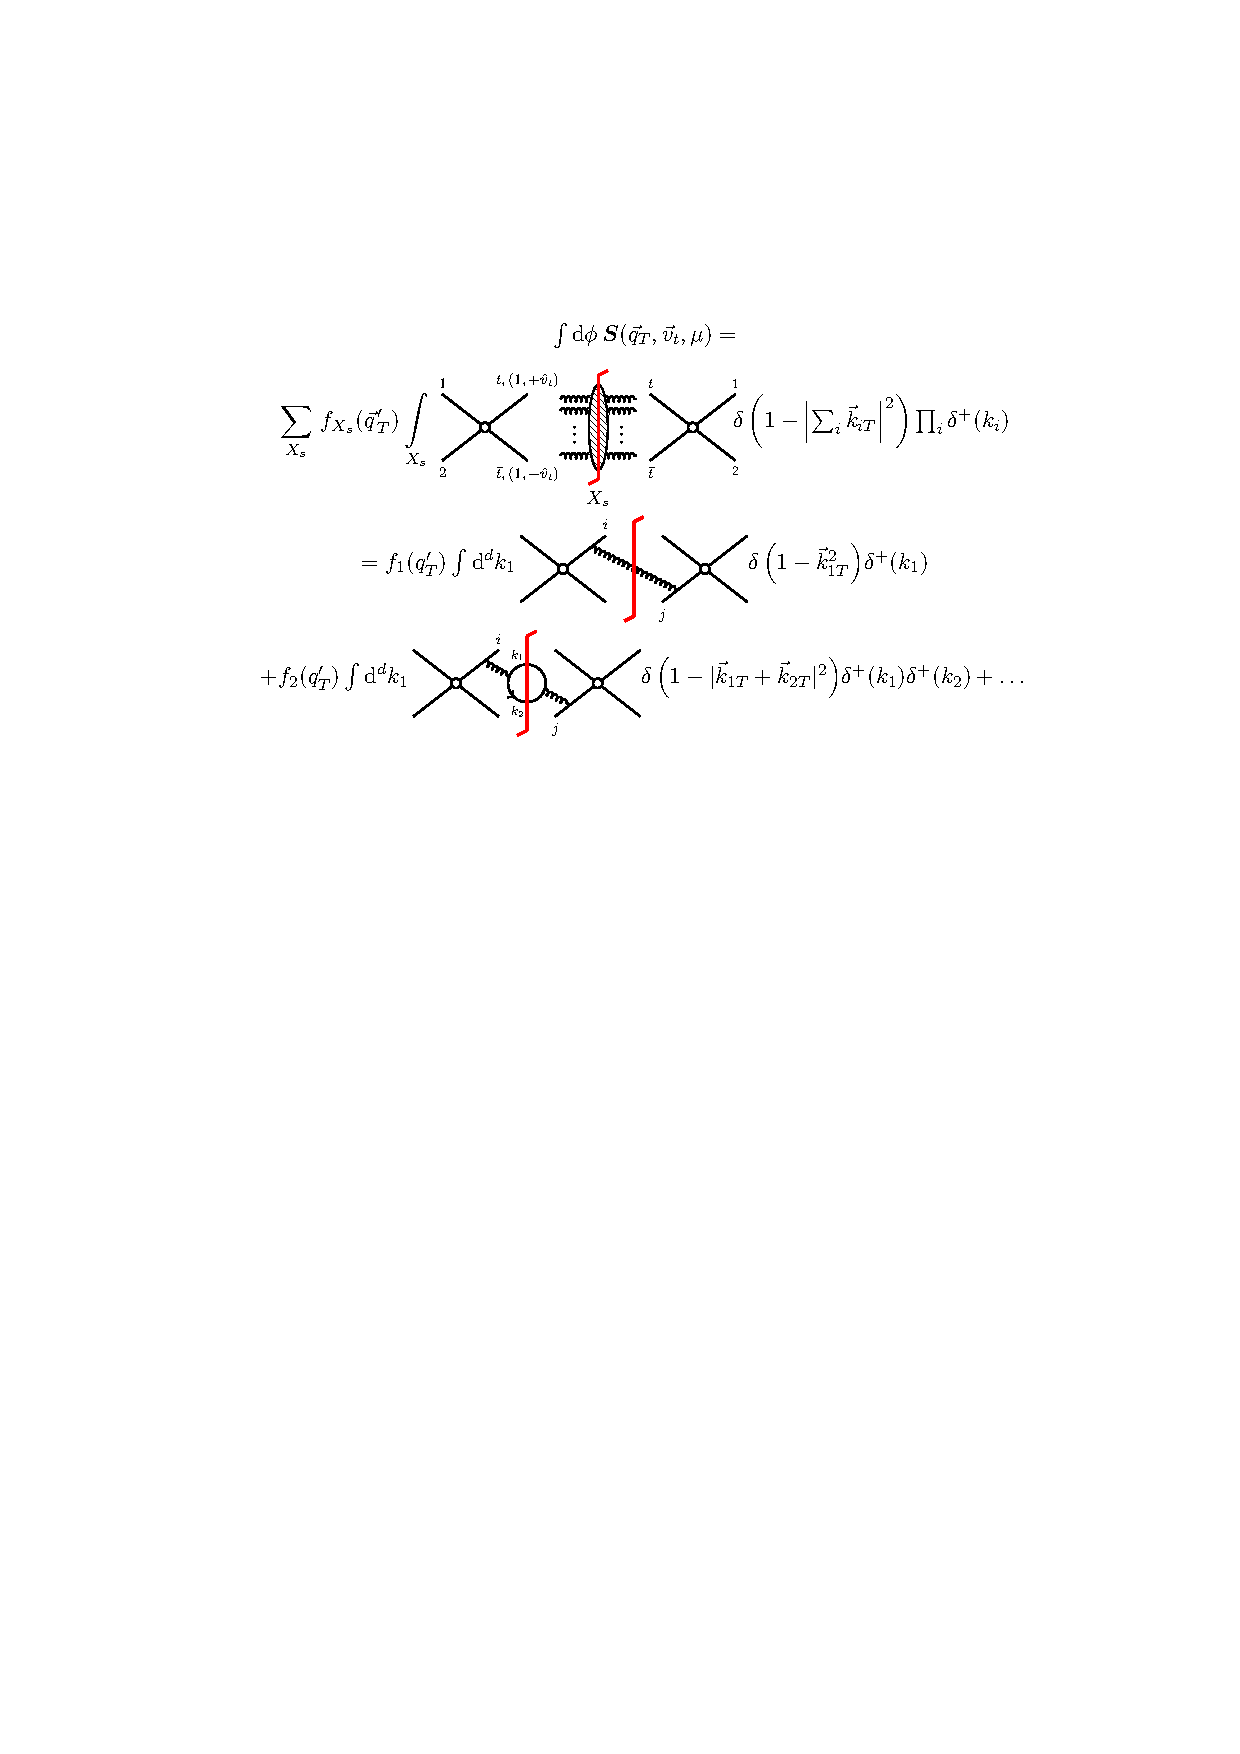
\includegraphics[scale=0.95]{fig1} }
\caption{Azimutally averaged soft function in momentum space. The sum over $X_s$ runs over all graphs that couple to the hard sub-process in the eikonal approximation, but with exact QCD interactions inside the hatched blob. The sum and product over $k_i$ runs over the cut (on-shell) emissions.  As explained in main text, the 
dependence on $q_T'$ has been factored out of the integration and is encoded by simple functions denoted by
$f_a(q_T')$.  The bottom rows illustrate particular graphs that contribute, respectively, at NLO and at NNLO. }
\label{fig:soft_function}
\end{figure}

Before the soft function can be evaluated, it is necessary to note that its individual constributions suffer from the so-called rapidity divergences associated to states that scale as $(\lambda^{\pm1},\lambda^{\mp1},1)$. Non-trivially, the rapidity divergences at NNLO can be regularised by means of the analytic regulator \cite{Li:2013mia, Becher:2011dz}, \emph{i.e.} by changing the integration measure as
\begin{align}
\dd^{4-2\epsilon} k_{i} \delta^{+}(k_i^2)\to \dd^{4-2\epsilon} k_{i} \delta^{+}(k_i^2) (k^+_i)^{-\alpha}~,
\end{align}
where $\alpha$ is a regulator analogous to $\epsilon$ in dimensional regularisation. Upon integration, the different graphs that contribute to the soft function can be expanded both in $\alpha$ and $\epsilon$. The $\alpha$ poles should canceled order by order in $\alpha_s$ and the $\epsilon$ poles should be canceled by the SCET renormalisation procedure, see below. 

%Two attractive features of this procedure is that preserve the gauge invariance of the soft function and that facilitates integration in dimensional regularisation by keeping many integrals scaleless. 

The graphs that appear in the evaluation of the soft function are not standard due to the presence of the delta function that constraint the $k_{iT}$ of the on-shell emissions, see Fig.~\ref{fig:soft_function}. 
At NNLO the soft function receives contributions from  double-cut (double-real) and single-cut (mixed real-virtual) graphs. The virtual loop in the latter can be integrated out using the results of Ref.~\cite{Bierenbaum:2011gg}. Due to this, below, we will focus on the double-cut graphs.

To integrate all the double-cut graphs we have designed, and automated, an algorithm to numerically integrate these. Non-trivially, this is possible because double-cut graphs share a common structure that can be exploited. The backbones of this algorithm are:
\begin{enumerate}
\item Identify all the divergences of every contribution  $G$ to the soft function and separate its integrand as 
 \begin{align}
G=  \int   \dd^d k_1 \dd^d k_2\, \, \frac{\delta^{+}(k_1)  \delta^{+}(k_2)} {(k_1^{+} k_2^+)^\alpha} 
\delta\left(1-|k_{1\perp}+k_{2\perp}|^2\right) \,  \mathcal{I}_G\times  \mathcal{W}_G, 
\end{align}
where the defining property of the weight part $\mathcal{W}_G$ is that it has at most integrable singularities. In contrast,  the infrared part $\mathcal{I}_G$ has divergences that, broadly speaking, gives rise to $\alpha$ and $\epsilon$ poles. 
\item Map the integration variables $\{k_i\}\to \{x_{ij}\}$ to a minimal number of domains $j$, each of which is a  unit hypercube ($x_{ij}\in [0,1]$) with singularities located only at zero. 
\item Implement sector decomposition to disentangle and factorises the 
$\alpha$ and $\epsilon$ poles of each graph. The entire sector decomposition procedure only depends on the details of  $\mathcal{I}_G$, and   $\mathcal{W}_G$ is treated as a weight function. This is crucial for efficiency reasons. After this point, $\alpha$ and $\epsilon$ expansion renders expressions of the form 
\begin{align}
G =\sum_j \sum_{r=-2,s=-3} \frac{1}{\alpha^r \epsilon^s}
 \int_{[0,1]^n} \dd^{n} \vec{x}\,\,  \mathcal{F}_{rsj} (\vec{x},\theta,\beta) ,
\end{align}
where now each integral on the right-hand-side is finite.
\item In general, such integrals are intricate but we have found that these are suitable for a numerical evaluation
using the CUBA library \cite{Hahn:2004fe}.
\end{enumerate}

\section{Validation of the integration strategy\label{sec:validation} }

In this section, we will describe a series of test of our numerical integration. 
Let us start by noting that the only graphs that are proportional to the number of light quark flavours, $n_f$, are those that involve emission of a fermion pair. Due to that, the cancellation of poles should occur independently for this set of graphs. To check this, let us denote by $G^{\text{fer}}_{ij}$ the graph in the third line of Fig.~\ref{fig:soft_function}. Only the contributions with $(i,j)$ set to   $\{(1,\txt),(2,\txt) ,(1,\txtb),(2,\txtb)
(\txt,\txtb), (\txt,\txt),  (\txtb,\txtb) \}$ are non-vanishing.

Both numerically and analytically, we have been able to compute all the poles of these graphs. Although, at intermediate steps, most integrals exhibit $\alpha$ poles, the only graphs that have these poles are
\begin{align}
\begin{gathered}
G^{\text{fer}}_{1t} = n_f  \Bf{T}_1\cdot \Bf{T}_t\left( \frac{c}{\alpha}+\dots\right), \qquad G^{\text{fer}}_{2t} = -n_f \Bf{T}_2\cdot \Bf{T}_t  \left( \frac{c}{\alpha}+\dots\right),\\
G^{\text{fer}}_{1\bar{t}} =n_f \Bf{T}_1\cdot \Bf{T}_{\bar{t}} \left( \frac{c}{\alpha}+\dots\right), 
\qquad G^{\text{fer}}_{2\bar{t}} = - n_f \Bf{T}_2\cdot \Bf{T}_{\bar{t}} \left( \frac{c}{\alpha}+\dots \right),
\end{gathered}
\end{align}
By using colour conservation one can show that the poles cancel when these graphs are added together. 
Indeed, this is what we find after combining all graphs
\begin{align}
\begin{gathered}
c (\text{analytically})= -\frac{8 }{3 \alpha \epsilon}-\frac{8 (3 \gamma_E +5-3 \log (2))}{9 \alpha}~,\\
c (\text{numerically})= -\frac{4.13}{\alpha} - 	\frac{2.66}{\alpha \epsilon} +\mathcal{O}(10^{-3})~.
\end{gathered}
\end{align}

After the cancellation of the $\alpha$ poles, the $\epsilon$ poles of the bare soft function must be canceled by the SCET renormalisation procedure 
\cite{Zhu:2012ts}:
\begin{align}
&  \Bf{S}(\mu) = \Bf{Z}^\dagger_s(\mu,\epsilon) \Bf{S}_{\text{bare}}(\epsilon)
  \Bf{Z}_s(\mu,\epsilon) 
\end{align}
Again, we have singled out all contributions proportional $n_f\alpha_s^2$ and confirmed that the $\Bf{Z}_s(\mu,\epsilon)$ operators remove all the $\epsilon$ poles of graphs involving the radiation of a fermion pair. 

\begin{figure}[ht!]
\centerline{
%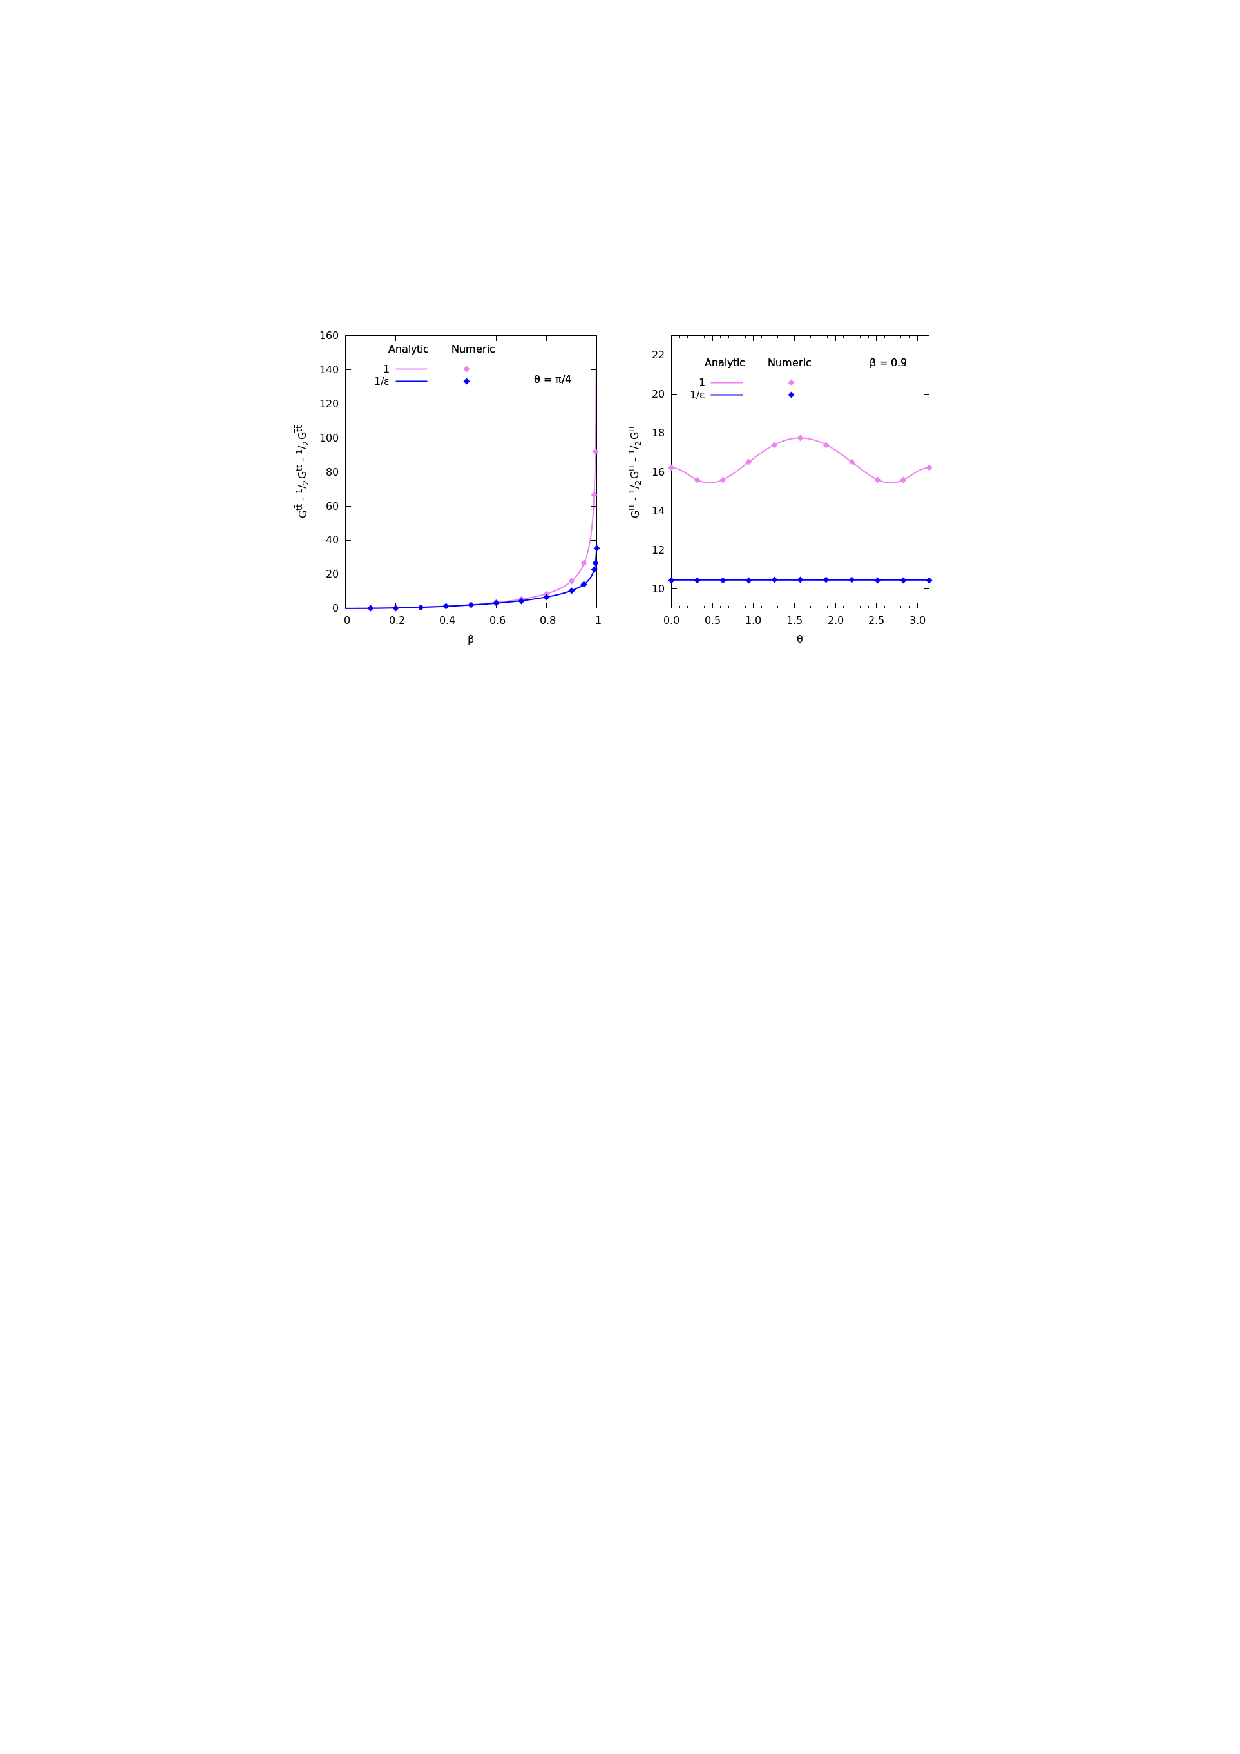
\includegraphics[scale=1]{fig2}
%\includegraphics[width=5.5cm]{./figsMTTD/bubble-theta34rene.png}
%\centering
\begin{tabular}{  c  c    }
	$a$  & $ a $ \\
\end{tabular}
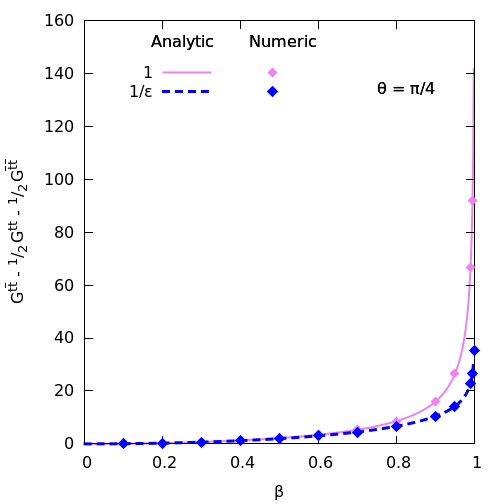
\includegraphics[width=6cm]{bubble-beta34rene.png}
\includegraphics[width=6cm]{bubble-theta34rene.png}
}
\caption{Numerical and analytic calculation of the kinematical part of 
$G^\text{fer}_{\ttb}- G^\text{fer}_{\txt\txt} /2- G^\text{fer}_{\txtb \txtb}$. Up to a global power of $q'_T$, the soft function only depends on the velocity $\beta$ and polar angle, $\theta$, of $p_\txt$.}
\label{fig:results}
\end{figure}

Within our numerical approach the graphs involving fermions are the most complicated. In spite of this, by means of  ordinary differential equations, we have been able to solve analytically such contributions up to order $\epsilon^0 \alpha^0$. Fig.~\ref{fig:results} shows the agreement between our numerical and analytic calculations for a particular combination of graphs. Analogous plots for other graphs can be found in \cite{sapeta}. This agreement holds with  absolute accuracy of order $10^{-3}$, which is the preliminary setting we used for the validation stage. 

\section{Conclusions}

Top pair cross-sections at NNLO can be evaluated by combining the
slicing method and SCET. The only missing result to apply this is the SCET soft function at NNLO  and we have 
developed an algorithm, based on sector decomposition, to evaluate all of its contributions.
 To validate this algorithm we focused on the part of the cross-section proportional to $\alpha_s^2 n_f$ and showed that the rapidity and infrared singularities cancel accordingly. Finally, by using ordinary differential equations, 
we also evaluated this part of the cross-section analytically and found 
perfect agreement with the numerical results, from our sector decomposition based algorithm. Thesefore, we conclude that the study presented in this proceedings constitutes a proof of concept of an approach that can be generalised to other processes at high orders. 


\section*{Acknowledgements}

We thank Mateusz Dobija for helping us to optimise our implementation of the CUBA library.  The project has received funding from the European Union's Horizon 2020
research  and  innovation  programme  under  the  Marie  Sk\l{}odowska-Curie
grant agreement NO. 665778.


\FloatBarrier

\begin{thebibliography}{99}
%\cite{Li:2013mia}
%% Applications

%\cite{Czakon:2015xqa}
\bibitem{Czakon:2015xqa} 
  M.~Czakon,
  %``Precision top-quark physics with applications,''
  Nucl.\ Part.\ Phys.\ Proc.\  {\bf 261-262}, 115 (2015).
  doi:10.1016/j.nuclphysbps.2015.03.010
  %%CITATION = doi:10.1016/j.nuclphysbps.2015.03.010;%%
  %1 citations counted in INSPIRE as of 02 Nov 2017


%%complete NNLO

%\cite{Czakon:2013goa}
\bibitem{Czakon:2013goa}
  M.~Czakon, P.~Fiedler and A.~Mitov,
  %``Total Top-Quark Pair-Production Cross Section at Hadron Colliders Through $O(?\frac{4}{S})$,''
  Phys.\ Rev.\ Lett.\  {\bf 110} (2013) 252004
  doi:10.1103/PhysRevLett.110.252004
  [arXiv:1303.6254 [hep-ph]].
  %%CITATION = doi:10.1103/PhysRevLett.110.252004;%%
  %933 citations counted in INSPIRE as of 28 Sep 2017

%\cite{Czakon:2017wor}
\bibitem{Czakon:2017wor}
  M.~Czakon, D.~Heymes, A.~Mitov, D.~Pagani, I.~Tsinikos and M.~Zaro,
  %``Top-pair production at the LHC through NNLO QCD and NLO EW,''
  arXiv:1705.04105 [hep-ph].
  %%CITATION = ARXIV:1705.04105;%%
  %9 citations counted in INSPIRE as of 28 Sep 2017

%\cite{Czakon:2015owf}
\bibitem{Czakon:2015owf}
  M.~Czakon, D.~Heymes and A.~Mitov,
  %``High-precision differential predictions for top-quark pairs at the LHC,''
  Phys.\ Rev.\ Lett.\  {\bf 116} (2016) no.8,  082003
  doi:10.1103/PhysRevLett.116.082003
  [arXiv:1511.00549 [hep-ph]].
  %%CITATION = doi:10.1103/PhysRevLett.116.082003;%%
  %99 citations counted in INSPIRE as of 28 Sep 2017


%% Partial NNLO

%\cite{Abelof:2015lna}
\bibitem{Abelof:2015lna}
  G.~Abelof, A.~Gehrmann-De Ridder and I.~Majer,
  %``Top quark pair production at NNLO in the quark-antiquark channel,''
  JHEP {\bf 1512} (2015) 074
  doi:10.1007/JHEP12(2015)074
  [arXiv:1506.04037 [hep-ph]].
  %%CITATION = doi:10.1007/JHEP12(2015)074;%%
  %19 citations counted in INSPIRE as of 28 Sep 2017
  
 %\cite{Abelof:2014jna}
\bibitem{Abelof:2014jna}
  G.~Abelof and A.~Gehrmann-De Ridder,
  %``Light fermionic NNLO QCD corrections to top-antitop production in the quark-antiquark channel,''
  JHEP {\bf 1412} (2014) 076
  doi:10.1007/JHEP12(2014)076
  [arXiv:1409.3148 [hep-ph]].
  %%CITATION = doi:10.1007/JHEP12(2014)076;%%
  %12 citations counted in INSPIRE as of 28 Sep 2017
  

%\cite{Bonciani:2015sha}
\bibitem{Bonciani:2015sha}
  R.~Bonciani, S.~Catani, M.~Grazzini, H.~Sargsyan and A.~Torre,
  %``The $q_T$ subtraction method for top quark production at hadron colliders,''
  Eur.\ Phys.\ J.\ C {\bf 75} (2015) no.12,  581
  doi:10.1140/epjc/s10052-015-3793-y
  [arXiv:1508.03585 [hep-ph]].
  %%CITATION = doi:10.1140/epjc/s10052-015-3793-y;%%
  %13 citations counted in INSPIRE as of 28 Sep 2017


%% Approximte NNLO

%\cite{Ahrens:2010zv}
\bibitem{Ahrens:2010zv}
  V.~Ahrens, A.~Ferroglia, M.~Neubert, B.~D.~Pecjak and L.~L.~Yang,
  %``Renormalization-Group Improved Predictions for Top-Quark Pair Production at Hadron Colliders,''
  JHEP {\bf 1009} (2010) 097
  doi:10.1007/JHEP09(2010)097
  [arXiv:1003.5827 [hep-ph]].
  %%CITATION = doi:10.1007/JHEP09(2010)097;%%
  %269 citations counted in INSPIRE as of 28 Sep 2017

%\cite{Ahrens:2011mw}
\bibitem{Ahrens:2011mw}
  V.~Ahrens, A.~Ferroglia, M.~Neubert, B.~D.~Pecjak and L.~L.~Yang,
  %``RG-improved single-particle inclusive cross sections and forward-backward asymmetry in $t\bar t$ production at hadron colliders,''
  JHEP {\bf 1109} (2011) 070
  doi:10.1007/JHEP09(2011)070
  [arXiv:1103.0550 [hep-ph]].
  %%CITATION = doi:10.1007/JHEP09(2011)070;%%
  %103 citations counted in INSPIRE as of 28 Sep 2017

%\cite{Kidonakis:2012rm}
\bibitem{Kidonakis:2012rm}
  N.~Kidonakis,
  %``NNLL threshold resummation for top-pair and single-top production,''
  Phys.\ Part.\ Nucl.\  {\bf 45} (2014) no.4,  714
  doi:10.1134/S1063779614040091
  [arXiv:1210.7813 [hep-ph]].
  %%CITATION = doi:10.1134/S1063779614040091;%%
  %114 citations counted in INSPIRE as of 28 Sep 2017

%\cite{Kidonakis:2014pja}
\bibitem{Kidonakis:2014pja}
  N.~Kidonakis,
  %``NNNLO soft-gluon corrections for the top-quark $p_T$ and rapidity distributions,''
  Phys.\ Rev.\ D {\bf 91} (2015) no.3,  031501
  doi:10.1103/PhysRevD.91.031501
  [arXiv:1411.2633 [hep-ph]].
  %%CITATION = doi:10.1103/PhysRevD.91.031501;%%
  %34 citations counted in INSPIRE as of 28 Sep 2017

%\cite{Gao:2012ja}
\bibitem{Gao:2012ja}
  J.~Gao, C.~S.~Li and H.~X.~Zhu,
  %``Top Quark Decay at Next-to-Next-to Leading Order in QCD,''
  Phys.\ Rev.\ Lett.\  {\bf 110} (2013) no.4,  042001
  doi:10.1103/PhysRevLett.110.042001
  [arXiv:1210.2808 [hep-ph]].
  %%CITATION = doi:10.1103/PhysRevLett.110.042001;%%
  %100 citations counted in INSPIRE as of 28 Sep 2017

%\cite{Brucherseifer:2013iv}
\bibitem{Brucherseifer:2013iv}
  M.~Brucherseifer, F.~Caola and K.~Melnikov,
  %``$\mathcal O(\alpha_s^2)$ corrections to fully-differential top quark decays,''
  JHEP {\bf 1304} (2013) 059
  doi:10.1007/JHEP04(2013)059
  [arXiv:1301.7133 [hep-ph]].
  %%CITATION = doi:10.1007/JHEP04(2013)059;%%
  %70 citations counted in INSPIRE as of 28 Sep 2017

%% qT subtraction 

%\cite{Catani:2007vq}
\bibitem{Catani:2007vq}
  S.~Catani and M.~Grazzini,
  %``An NNLO subtraction formalism in hadron collisions and its application to Higgs boson production at the LHC,''
  Phys.\ Rev.\ Lett.\  {\bf 98} (2007) 222002
  doi:10.1103/PhysRevLett.98.222002
  [hep-ph/0703012].
  %%CITATION = doi:10.1103/PhysRevLett.98.222002;%%
  %517 citations counted in INSPIRE as of 28 Sep 2017


%? Soft current
%\cite{Bierenbaum:2011gg}
\bibitem{Bierenbaum:2011gg}
  I.~Bierenbaum, M.~Czakon and A.~Mitov,
  %``The singular behavior of one-loop massive QCD amplitudes with one external soft gluon,''
  Nucl.\ Phys.\ B {\bf 856} (2012) 228
  doi:10.1016/j.nuclphysb.2011.11.002
  [arXiv:1107.4384 [hep-ph]].
  %%CITATION = doi:10.1016/j.nuclphysb.2011.11.002;%%
  %48 citations counted in INSPIRE as of 28 Sep 2017


%% Small qT SCET factorisation

%\cite{Becher:2014oda}
\bibitem{Becher:2014oda} 
  T.~Becher, A.~Broggio and A.~Ferroglia,
  %``Introduction to Soft-Collinear Effective Theory,''
  Lect.\ Notes Phys.\  {\bf 896}, pp.1 (2015)
  doi:10.1007/978-3-319-14848-9
  [arXiv:1410.1892 [hep-ph]].
  %%CITATION = doi:10.1007/978-3-319-14848-9;%%
  %68 citations counted in INSPIRE as of 31 Oct 2017


\bibitem{Li:2013mia} 
  H.~T.~Li, C.~S.~Li, D.~Y.~Shao, L.~L.~Yang and H.~X.~Zhu,
  %``Top quark pair production at small transverse momentum in hadronic collisions,''
  Phys.\ Rev.\ D {\bf 88}, 074004 (2013)
  doi:10.1103/PhysRevD.88.074004
  [arXiv:1307.2464 [hep-ph]].
  %%CITATION = doi:10.1103/PhysRevD.88.074004;%%
  %38 citations counted in INSPIRE as of 28 Sep 2017
 
 %\cite{Zhu:2012ts}
\bibitem{Zhu:2012ts} 
  H.~X.~Zhu, C.~S.~Li, H.~T.~Li, D.~Y.~Shao and L.~L.~Yang,
  %``Transverse-momentum resummation for top-quark pairs at hadron colliders,''
  Phys.\ Rev.\ Lett.\  {\bf 110}, no. 8, 082001 (2013)
  doi:10.1103/PhysRevLett.110.082001
  [arXiv:1208.5774 [hep-ph]].
  %%CITATION = doi:10.1103/PhysRevLett.110.082001;%%
  %33 citations counted in INSPIRE as of 28 Sep 2017
 
 %%%%%%%%%%%%%%%%%%%%%%%%%%%
 %% Hard function 
  
  %\cite{Baernreuther:2013caa}
\bibitem{Baernreuther:2013caa}
  P.~B�rnreuther, M.~Czakon and P.~Fiedler,
  %``Virtual amplitudes and threshold behaviour of hadronic top-quark pair-production cross sections,''
  JHEP {\bf 1402} (2014) 078
  doi:10.1007/JHEP02(2014)078
  [arXiv:1312.6279 [hep-ph]].
  %%CITATION = doi:10.1007/JHEP02(2014)078;%%
  %29 citations counted in INSPIRE as of 28 Sep 2017
  
  %\cite{Gehrmann:2012ze}
\bibitem{Gehrmann:2012ze}
  T.~Gehrmann, T.~Lubbert and L.~L.~Yang,
  %``Transverse parton distribution functions at next-to-next-to-leading order: the quark-to-quark case,''
  Phys.\ Rev.\ Lett.\  {\bf 109} (2012) 242003
  doi:10.1103/PhysRevLett.109.242003
  [arXiv:1209.0682 [hep-ph]].
  %%CITATION = doi:10.1103/PhysRevLett.109.242003;%%
  %47 citations counted in INSPIRE as of 28 Sep 2017
  
  %\cite{Gehrmann:2014yya}
\bibitem{Gehrmann:2014yya}
  T.~Gehrmann, T.~Luebbert and L.~L.~Yang,
  %``Calculation of the transverse parton distribution functions at next-to-next-to-leading order,''
  JHEP {\bf 1406} (2014) 155
  doi:10.1007/JHEP06(2014)155
  [arXiv:1403.6451 [hep-ph]].
  %%CITATION = doi:10.1007/JHEP06(2014)155;%%
  %57 citations counted in INSPIRE as of 28 Sep 2017
  
   %%%%%%%%%%%%%%%%%%%%%%%%%%%
 %% Numerical integration 
  
  %\cite{Hahn:2004fe}
\bibitem{Hahn:2004fe}
  T.~Hahn,
  %``CUBA: A Library for multidimensional numerical integration,''
  Comput.\ Phys.\ Commun.\  {\bf 168} (2005) 78
  doi:10.1016/j.cpc.2005.01.010
  [hep-ph/0404043].
  %%CITATION = doi:10.1016/j.cpc.2005.01.010;%%
  %385 citations counted in INSPIRE as of 28 Sep 2017
  
  %%Analytic
  
  %\cite{Becher:2011dz}
\bibitem{Becher:2011dz}
  T.~Becher and G.~Bell,
  %``Analytic Regularization in Soft-Collinear Effective Theory,''
  Phys.\ Lett.\ B {\bf 713} (2012) 41
  doi:10.1016/j.physletb.2012.05.016
  [arXiv:1112.3907 [hep-ph]].
  %%CITATION = doi:10.1016/j.physletb.2012.05.016;%%
  %47 citations counted in INSPIRE as of 28 Sep 2017

  %% 
  %\cite{Dittmaier:2007wz}

\bibitem{Dittmaier:2007wz}
  S.~Dittmaier, P.~Uwer and S.~Weinzierl,
  %``NLO QCD corrections to t anti-t + jet production at hadron colliders,''
  Phys.\ Rev.\ Lett.\  {\bf 98} (2007) 262002
  doi:10.1103/PhysRevLett.98.262002
  [hep-ph/0703120 [HEP-PH]].
  %%CITATION = doi:10.1103/PhysRevLett.98.262002;%%
  %256 citations counted in INSPIRE as of 28 Sep 2017
  
  %\cite{Dittmaier:2008uj}
\bibitem{Dittmaier:2008uj}
  S.~Dittmaier, P.~Uwer and S.~Weinzierl,
  %``Hadronic top-quark pair production in association with a hard jet at next-to-leading order QCD: Phenomenological studies for the Tevatron and the LHC,''
  Eur.\ Phys.\ J.\ C {\bf 59} (2009) 625
  doi:10.1140/epjc/s10052-008-0816-y
  [arXiv:0810.0452 [hep-ph]].
  %%CITATION = doi:10.1140/epjc/s10052-008-0816-y;%%
  %144 citations counted in INSPIRE as of 28 Sep 2017
  
    %\cite{sapeta}
\bibitem{sapeta}
  S.~Sapeta, Proceedings of the
  %``Hadronic top-quark pair production in association with a hard jet at next-to-leading order QCD: Phenomenological studies for the Tevatron and the LHC,''
  13th International Symposium on Radiative Corrections  (RADCOR), PoS 2017.
  %%CITATION = doi:10.1140/epjc/s10052-008-0816-y;%%
  %144 citations counted in INSPIRE as of 28 Sep 2017
  

   \end{thebibliography}


\end{document}

